\documentclass[border=2pt]{standalone}
\usepackage{amsmath}
\usepackage{tikz}
\usetikzlibrary{intersections}
\usetikzlibrary{arrows}
\usetikzlibrary{quotes,angles}
\usepackage{amsmath}
\usepackage{xcolor}

\begin{document}

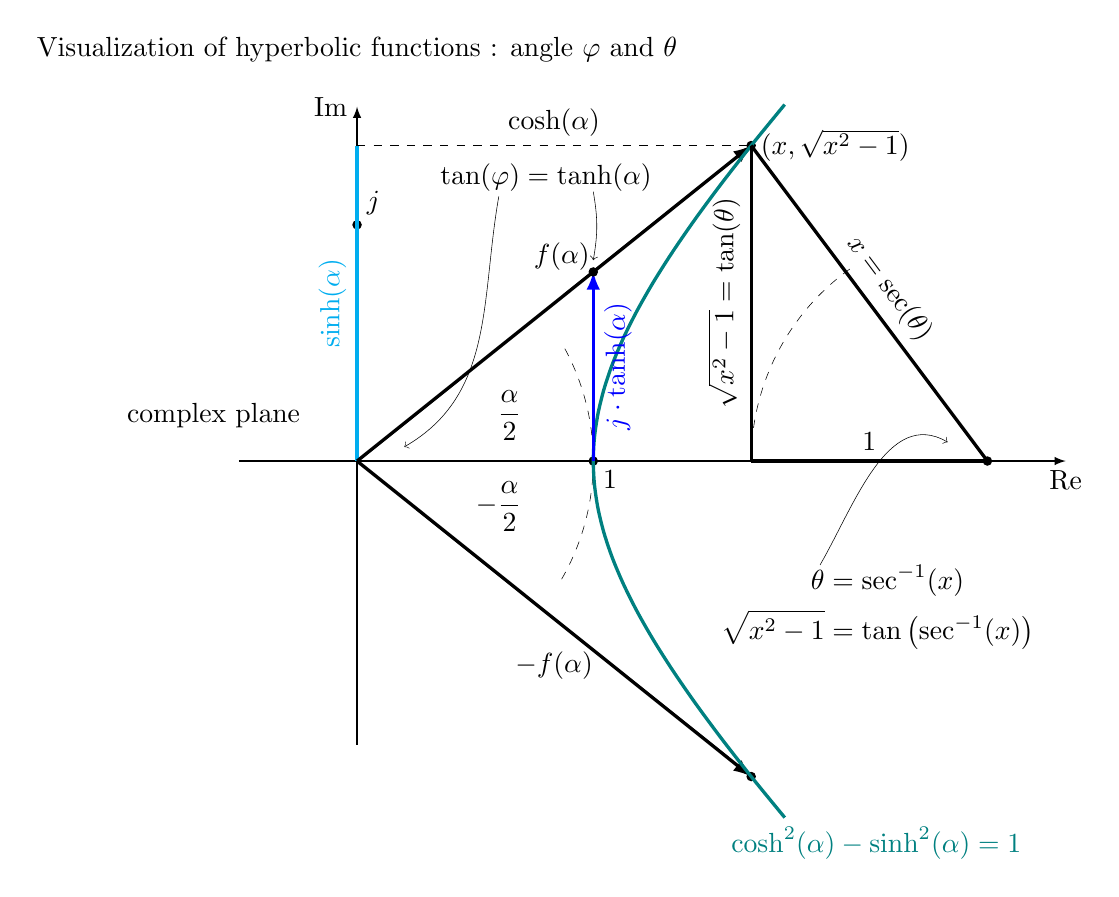
\begin{tikzpicture}[scale=3.0]

% Draw x and y axis lines
\draw [->,>=latex] (-0.5,0) -- (3.00,0) node [below] {$\mathrm{Re}$};
\draw [->,>=latex] (0,-1.2) -- (0,1.50) node [left ] {$\mathrm{Im}$};
\node[above left] at (-0.2, 0.1) {complex plane};
\filldraw[black] (1,0) circle (0.5pt) node[below right] {$1$} ;
\filldraw[black] (0,1) circle (0.5pt) node[above right] {$j$} ;
\node[above] at (0.0,1.65) {Visualization of hyperbolic functions : angle $\varphi$ and $\theta$};

% Draw a circle at the origin of radius 1
%\draw (0,0) circle (1);
\draw [very thin, dashed] ({cos(-30)},{sin(-30)}) arc (-30:30:1) ;

%\draw [very thin, dashed] (-1.5,-1.5) -- ( 1.5, 1.5) node[above] {$y=x$} ;
%\draw [very thin, dashed] (-1.5, 1.5) -- ( 1.5,-1.5) ;

\pgfmathsetmacro{\angle}{1.1}
\pgfmathsetmacro{\length}{\angle}
\pgfmathsetmacro{\anglevarphi}{atan(tanh(\angle))}
\pgfmathsetmacro{\angletheta}{acos(1/cosh(\angle))}

\filldraw[black] ({ cosh(\angle)}, { sinh(\angle)}) circle (0.5pt) node[right] {$(x,\sqrt{x^2-1})$} ;
\filldraw[black] ({ cosh(\angle)}, {-sinh(\angle)}) circle (0.5pt) ;

\draw [very thin, dashed] ( 0.0, { sinh(\angle)}) -- node[above] {$\cosh(\alpha)$}  ({ cosh(\angle)}, { sinh(\angle)}) ;
\draw [very thick, cyan] ( 0.0, 0.0) -- node[above, rotate=90] {$\sinh(\alpha)$}  ( 0.0, { sinh(\angle)}) ;

\draw[very thick, ->,>=latex] (0,0) -- node[above=8pt] {$\;\;f(\alpha)$} ({ cosh(\angle)}, { sinh(\angle)}) ;
\draw[very thick, ->,>=latex] (0,0) -- node[below=8pt] {$-f(\alpha)$} ({ cosh(\angle)}, {-sinh(\angle)}) ;



% 画双曲线
\draw[very thick,smooth,variable=\x, teal] plot[domain=-\angle-0.1:\angle+0.1] ({ cosh(\x)}, {sinh(\x)}) ;
\node[below right, teal] at ({ cosh(\angle-0.1)}, {-sinh(\angle+0.1)}) {$\cosh^2(\alpha) - \sinh^2(\alpha) = 1$} ;
%\draw[very thick,smooth,variable=\x, teal] plot[domain=-1.2:1.2] ({-cosh(\x)}, {sinh(\x)}) ;

\draw[very thick] ({ cosh(\angle)}, 0) -- node[above , rotate=90] {$\sqrt{x^2-1}=\tan(\theta)$} ({ cosh(\angle)}, { sinh(\angle)}) ;
\draw[very thick, ->,>=latex, blue] ( 1, 0) -- node[below , rotate=90] {$j\cdot\tanh(\alpha)$} ( 1, { tanh(\angle)}) ;

\node[above=4pt ] at (0.6, 0) {$\;\;\:\dfrac{\alpha}{2}$} ;
\node[below=4pt ] at (0.6, 0) {$ -\dfrac{\alpha}{2}$} ;

\filldraw[black] ( 1, { tanh(\angle)}) circle (0.5pt) ;
\draw [very thin, ->] (0.8, 1.1) node[above ] {$\tan(\varphi) = \tanh(\alpha)$} (1.0, 1.14) to [out=280,in=80] ( 1, { tanh(\angle) + 0.05}) ;
\draw [very thin, ->] (0.60, 1.12) to [out=260,in=30] (0.20, 0.06) ;

\begin{scope}[shift={({ cosh(\angle)}, { sinh(\angle)})}]
\draw [very thick, rotate=-\angletheta] (0, 0) -- node[above, rotate=-\angletheta] {$x=\sec(\theta)$} ({ cosh(\angle)}, 0)  ;
\end{scope}

\begin{scope}[shift={({ cosh(\angle)}, 0)}]
\draw [very thick] (0, 0) -- node[above] {$1$} ( 1, 0)  ;
\filldraw[black] ( 1, 0) circle (0.5pt) ;
\draw [very thin, dashed] (0,0) arc (180:125:1) ;
\end{scope}

\node[below right] at (1.50,-0.40) {$
\begin{aligned}
\theta & =\sec^{-1}(x)\\
\sqrt{x^{2}-1} & =\tan\left(\sec^{-1}(x)\right)
\end{aligned}
$};

\draw [very thin, ->] (1.96,-0.44) to [out=60,in=150] (2.5, 0.08) ;

\end{tikzpicture}

\end{document}
